% Project report template. Placeholders in double angle brackets are filled from Project-Report/evidence by build_latex.py.
\documentclass[11pt,a4paper]{article}

\usepackage[T1]{fontenc}
\usepackage[utf8]{inputenc}
\usepackage{lmodern}
\usepackage[english]{babel}
\usepackage{microtype}
\usepackage[margin=2.4cm]{geometry}
\usepackage{setspace}
\usepackage{graphicx}
\usepackage{booktabs}
\usepackage{longtable}
\usepackage{array}
\usepackage{enumitem}
\usepackage{float}
\usepackage{amsmath}
\usepackage{xcolor}
\usepackage{fancyhdr}
\usepackage{caption}
\usepackage{titlesec}
\usepackage[hidelinks]{hyperref}

\definecolor{heading}{HTML}{1B3A66}
\titleformat{\section}{\Large\bfseries\color{heading}}{\thesection.}{0.6em}{}
\titleformat{\subsection}{\large\bfseries\color{heading}}{\thesubsection}{0.6em}{}
\titlespacing*{\section}{0pt}{1.6em}{0.6em}
\titlespacing*{\subsection}{0pt}{1.2em}{0.4em}

\setstretch{1.08}
\setlength{\parskip}{0.55em}
\setlength{\parindent}{0pt}
\setlist{itemsep=0.25em,topsep=0.3em}
\captionsetup{font=small,labelfont=bf,skip=6pt}
\renewcommand{\arraystretch}{1.18}

\pagestyle{fancy}
\fancyhf{}
\lhead{\small Shahoud Shahid, 23i-2515}
\rhead{\small DS3003 \& DS3004 Project Report}
\cfoot{\small\thepage}
\renewcommand{\headrulewidth}{0.3pt}

\newcommand{\code}[1]{\texttt{\detokenize{#1}}}

\hypersetup{pdftitle={Building and Analysing a Near-Real-Time and Periodic Data Warehouse for a Retail Chain},
            pdfauthor={Shahoud Shahid}}

\begin{document}

% ------------------------------------------------------------------ cover
\begin{titlepage}
\thispagestyle{empty}
\centering
\vspace*{3cm}
{\large National University of Computer and Emerging Sciences\par}
\vspace{0.3cm}
{\large FAST-NUCES\par}
\vspace{1.2cm}
{\normalsize DS3003 \& DS3004: Data Warehousing \& Business Intelligence\par}
{\normalsize Fall 2026\par}
\vspace{1.6cm}
{\Huge\bfseries\color{heading} Building and Analysing a Near-Real-Time and Periodic Data Warehouse for a Retail Chain\par}
\vspace{1.2cm}
{\large Project Report\par}
\vspace{1.6cm}
{\Large\bfseries Shahoud Shahid\par}
\vspace{0.3cm}
Roll number: 23i-2515\par
Section: DS-A\par
\vspace{1.2cm}
13 November 2026\par
\end{titlepage}

% ------------------------------------------------------------------ 1
\section{Project Overview}

This project builds and analyses a data warehouse for a retail chain that sells on its website and in physical stores. Online sales must reach the warehouse shortly after they happen, while store sales arrive once an hour. Both come from one public file of real transactions, the UCI Online Retail dataset, which runs from 1 December 2010 to 9 December 2011 \cite{chen}. The file contains no Master Data, so the program builds it from fixed rules.

The work consists of a Python program and a MySQL star schema. The program cleans the file, builds the Master Data, splits the transactions into an online stream and periodic groups, and starts three independent threads. MESHJOIN \cite{polyzotis}, a stream-relation join, adds the customer and product attributes held on disk to each transaction. The enriched rows are loaded into the warehouse, and 20 OLAP queries are then run against it.

The optional bonus is also implemented: Live results are written to a cache table first and move into the warehouse during a slow period. Every measured figure in this report comes from one official run at the settings given in the assignment, on MySQL <<e:server_version>>.

% ------------------------------------------------------------------ 2
\section{Data Warehouse Schema}
\label{sec:schema}

\begin{figure}[ht]
  \centering
  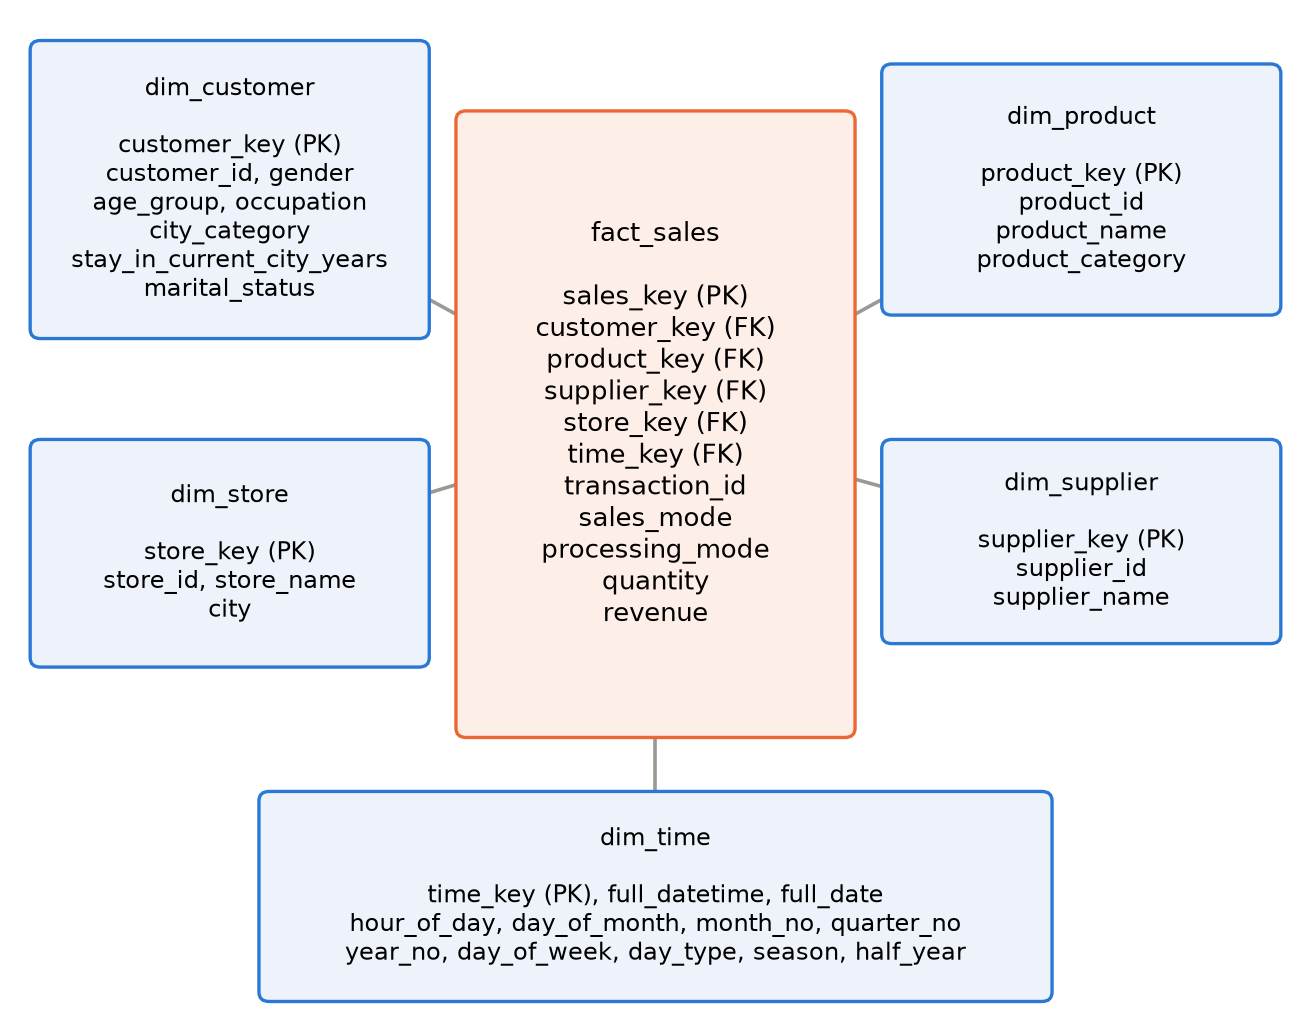
\includegraphics[width=0.92\textwidth]{figures/star.png}
  \caption{The star schema. Each dimension joins the fact table through a surrogate key created for this project.}
  \label{fig:star}
\end{figure}

The fact table sits at the centre of Figure~\ref{fig:star} and holds one tuple per transaction: one product in one shopping cart, with one customer, store, supplier and time. This is the finest grain the data offers, and the queries need it, because Q16 and Q19 work on individual transactions. Totals are calculated in SQL and are never stored in a second fact table.

The two measures are quantity and revenue. Revenue ($\mathrm{SALE} = \mathrm{quantity} \times \mathrm{price}$) is in neither the transactional file nor the Master Data, so it is calculated when the tuple is consolidated. The primary key is a surrogate, \code{sales_key}, because the pair \code{(transaction_id, product_id)} is not unique: 19,157 cleaned rows share that pair with another row, and a unique constraint on it would silently drop them. The column \code{transaction_id} stays on the fact table as a degenerate dimension, since Q16 counts shopping carts with it.

The fact table has five foreign keys, to customer, product, supplier, store and time. Supplier joins through the fact table rather than through product, which keeps the design a star and not a snowflake. Every dimension keeps the original ids, stored with a binary collation so that MySQL compares them exactly as Python does. In the time dimension, \code{time_key} has the form YYYYMMDDHHMM, with one row per distinct event time. Its parts are stored as separate columns (date, hour, day of month, month, quarter, year, day of week, weekday or weekend, season and half-year) so that queries can group by them without re-reading the timestamp.

The script \code{Create-DW/create_dw.sql} first drops the view \code{STORE_QUARTERLY_SALES}, the fact table and the dimensions, in dependency order. It then recreates them with their primary keys, foreign keys and \texttt{CHECK} constraints. It also creates the working tables, which have no foreign keys into the warehouse: \code{customer_master_data}, \code{product_master_data}, \code{periodic_sales_data}, \code{shed_table} and \code{live_cache}, together with tables for logs, rejects and recovery.

% ------------------------------------------------------------------ 3
\section{Data Preparation and Cleaning Counts}

The program does all the cleaning itself, with no manual edits to the file. A transaction is kept only if its quantity and unit price are both above zero, it has a customer ID, and its \code{transaction_id} does not start with the letter C.

\begin{table}[ht]
  \centering
  \caption{Transactions before and after cleaning.}
  \begin{tabular}{lr}
    \toprule
    Count & Transactions \\
    \midrule
    Before cleaning & 541,909 \\
    After cleaning & 397,884 \\
    Removed & 144,025 \\
    Failed: cancellation (id starts with C) & 9,288 \\
    Failed: quantity not above zero & 10,624 \\
    Failed: unit price not above zero & 2,517 \\
    Failed: customer ID missing & 135,080 \\
    \bottomrule
  \end{tabular}
\end{table}

A row can fail more than one test, so the four failure counts add up to more than the number removed. After cleaning there are 18,532 shopping carts, 4,338 customers and 3,665 products.

Two details decide whether the rules work at all. First, the id columns mix integers and strings and the customer column has blanks, so a default spreadsheet read turns 17850 into 17850.0. That changes the MD5 of the id and, with it, every attribute of every customer. The program therefore reads the raw values and converts each id to exact text. Second, the cleaning tests in the assignment form a closed list, so the 5,194 exact duplicate rows stay in as separate transactions.

% ------------------------------------------------------------------ 4
\section{The \texorpdfstring{\texttt{sales\_mode}}{sales\_mode} Rule and the Store Rule}

The file does not say where each cart was bought, so a fixed rule decides this from the invoice number. Every line in a cart receives the same result. Let $h(t)$ be the first eight hexadecimal characters of the MD5 of the UTF-8 text $t$, read as an integer. Then
\begin{equation}
  r(t) = h(t) \bmod 10,
  \qquad
  \text{sales mode} =
  \begin{cases}
    \text{online} & r(t) \in \{0,\dots,6\},\\
    \text{physical store} & r(t) \in \{7,8,9\}.
  \end{cases}
  \label{eq:mode}
\end{equation}
A store cart takes its store from the same number, while online carts use store 1:
\begin{equation}
  \mathrm{store\_id}(t) = 2 + \bigl(h(t) \bmod 4\bigr).
  \label{eq:store}
\end{equation}

\begin{table}[ht]
  \centering
  \caption{Worked examples of Equations~\ref{eq:mode} and~\ref{eq:store}.}
  \begin{tabular}{lllll}
    \toprule
    \code{transaction_id} & First 8 hex & As integer & mod 10 & Result \\
    \midrule
    536365 & 3e6d49ce & 1047349710 & 0 & Online, store 1 \\
    536370 & 2d918f31 & 764514097  & 7 & Physical; mod 4 = 1, store 3 \\
    \bottomrule
  \end{tabular}
\end{table}

The rule produced 278,740 online transactions (70.06\%) and 119,144 periodic ones (29.94\%), in line with the 70 and 30 percent the assignment expects.

The store rule has a side effect that matters when reading store results. Both remainders come from the same number, so they are not independent. Remainders 7 and 9 are odd, and an odd number modulo 4 is always 1 or 3, so those carts can only reach stores 3 and 5. Remainder 8 is even, so those carts can only reach stores 2 and 4. Two of the three store remainders therefore feed just two stores each.

\begin{table}[ht]
  \centering
  \caption{Shopping carts per physical store.}
  \begin{tabular}{llr}
    \toprule
    Store & Name & Carts \\
    \midrule
    2 & London Bridge & 909 \\
    3 & Manchester Arndale & 1,869 \\
    4 & Birmingham Bullring & 920 \\
    5 & Edinburgh Princes & 1,863 \\
    \bottomrule
  \end{tabular}
\end{table}

Manchester and Edinburgh therefore receive roughly twice as many carts as London and Birmingham. This follows from the arithmetic of the rule and does not reflect real trade, so the store comparisons in Q12, Q13, Q15 and Q20 should not be read as a measure of store performance.

% ------------------------------------------------------------------ 5
\section{MESHJOIN}

MESHJOIN was introduced by Polyzotis et al.\ in 2008 to join a stream with a relation during the transformation phase of ETL \cite{polyzotis}. The stream $S$ is the sequence of transactions, and the relation $R$ is the Master Data, which stays on disk because it is treated as too large to load into memory. Looking up $R$ once per transaction would require many random reads, and the join would fall behind the stream. Waiting for each hour to close would stall the stream instead. MESHJOIN avoids both problems by reading $R$ cyclically, one partition at a time, and joining each partition with all the transactions currently in memory.

\begin{figure}[ht]
  \centering
  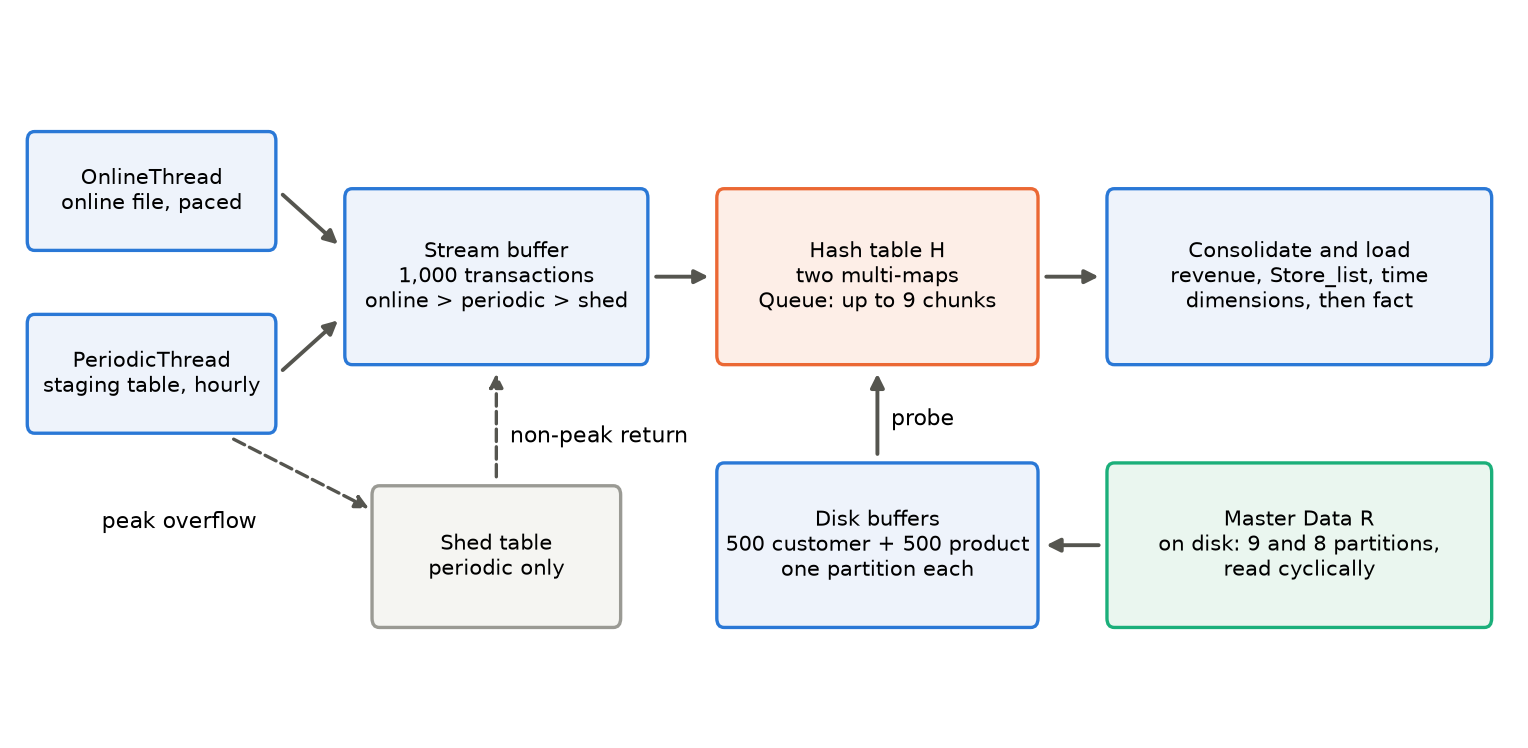
\includegraphics[width=\textwidth]{figures/meshjoin.png}
  \caption{The MESHJOIN pipeline as implemented. Dashed arrows are the load-shedding path.}
  \label{fig:meshjoin}
\end{figure}

\subsection{Components}

\begin{table}[ht]
  \centering
  \caption{The MESHJOIN components as implemented.}
  \begin{tabular}{@{}>{\raggedright\arraybackslash}p{3.0cm}>{\raggedright\arraybackslash}p{11.8cm}@{}}
    \toprule
    Component & In this program \\
    \midrule
    Stream buffer & Holds up to 1,000 transactions while MESHJOIN finishes an iteration. Three lanes share that space and are read in priority order: online, periodic, shed. \\
    Hash table $H$ & A multi-map of the transactions in memory, with two indexes over the same objects (by \code{customer_id} and by \code{product_id}), since there are two join attributes. \\
    Queue & Keeps a reference to each chunk in arrival order, oldest at the end. It never copies a transaction. \\
    Disk buffer & One per Master Data table, holding a single partition of at most 500 tuples. The next iteration overwrites it. \\
    Master Data $R$ & Two MySQL tables, read by key range 500 tuples at a time in an endless cycle. Nothing is cached. \\
    \bottomrule
  \end{tabular}
\end{table}

\subsection{One iteration}

\begin{enumerate}
  \item Read the next partition of each Master Data table into its disk buffer, wrapping back to the first after the last.
  \item Move up to 500 transactions from the stream buffer into $H$ as one chunk, and add its pointer to the queue.
  \item Probe $H$ with the join attribute of each Master Data tuple in the disk buffers. The customer pass adds the customer attributes, and the product pass adds the product and supplier. The store is not part of the join: it comes from the in-memory \code{Store_list} when the row is consolidated.
  \item Remove the oldest chunk once it has been compared with all of both tables.
\end{enumerate}

\subsection{Partitions, and how long a chunk stays}

\begin{table}[ht]
  \centering
  \caption{Master Data partitions, counted from the loaded tables.}
  \begin{tabular}{lrrr}
    \toprule
    Master Data table & Tuples & Partitions & Tuples in last partition \\
    \midrule
    Customer & <<n:master_data.customers>> & <<n:master_data.customer_partitions>> & 338 \\
    Product  & <<n:master_data.products>>  & <<n:master_data.product_partitions>>  & 165 \\
    \bottomrule
  \end{tabular}
\end{table}

The assignment expects about six product partitions but asks for the count to come from the loaded table. The cleaned file has 3,665 distinct products, which makes eight. Because the two cycles have different lengths, a chunk stays for the longer one, nine iterations. That way it meets all nine customer partitions and all eight product partitions, wherever the two cursors were when it entered. On its ninth iteration it meets one product partition a second time, which sets the same values again. Removing the chunk one iteration earlier would lose matches, and a test confirms this by building a row whose partition is seen last.

\subsection{Threads and modes}

The system runs on three independent threads that do not take turns. \texttt{OnlineThread} reads the online file at an adjustable speed. \texttt{PeriodicThread} keeps the simulated clock and extracts one group each hour. \texttt{MeshJoinThread} runs the four steps and the load shedding, and it is the only thread that writes to the warehouse. While the program runs, the commands \code{online}, \code{periodic}, \code{both}, \code{peak}, \code{non-peak}, \code{status} and \code{quit} change its behaviour.

% ------------------------------------------------------------------ 6
\section{Three Shortcomings of MESHJOIN}

\subsection{A fixed wait, even when the match is found early}

Every transaction stays for a full cycle of the Master Data, nine iterations here, even if both of its matches turned up in the first. The Master Data keys are unique, so nothing more can arrive, but the algorithm has no way to use that. In the official run the median Live latency was <<n:live_latency_ms.p50_of_hours_median>>~ms and the median 95th percentile was <<n:live_latency_ms.p95_of_hours_median>>~ms. About 1.8 seconds of that is this fixed cycle, at the minimum iteration time of 200~ms. The cost also grows with the Master Data: doubling $R$ doubles the wait.

\subsection{No adaptation to skew}

The cyclic scan reads every partition equally often, whatever the stream needs. Demand in this data is uneven: the busiest 10\% of products account for <<n:skew.products.top_decile_share_pct>>\% of transactions, and the busiest 10\% of customers for <<n:skew.customers.top_decile_share_pct>>\%. A tuple wanted by hundreds of transactions costs the same disk read as one that nobody wants. Later algorithms such as HYBRIDJOIN use an index and key frequencies to fetch what is needed sooner.

\subsection{Fragile under bursts}

The stream buffer and chunk size are fixed, so the join responds to the shape of the arrivals and not only to their rate. The average iteration took <<n:iteration_ms_weighted_average>>~ms, which gives far more capacity than the average arrival of about 121 transactions per second (80 online plus about 41 periodic). Even so, each hourly release of about 2,480 rows cannot fit in a 1,000-slot buffer, so rows are shed at peak although there is spare capacity a moment later. Anything in the buffer or in $H$ is also lost if the program crashes. This project handles that with a recovery log, which is extra machinery that MESHJOIN does not provide on its own.

% ------------------------------------------------------------------ 7
\section{Periodic Groups}

The periodic transactions are sorted by \code{event_time} and split into 48 groups of equal count, with group 0 at the first hour and group 47 at the last. A \code{released} flag in the staging table ensures that no transaction is extracted twice.

\begin{table}[ht]
  \centering
  \caption{Sizes of the 48 periodic groups.}
  \begin{tabular}{lr}
    \toprule
    Group measure & Transactions \\
    \midrule
    Total periodic transactions & 119,144 \\
    Smallest group & <<n:groups.smallest>> \\
    Largest group & <<n:groups.largest>> \\
    Groups of 2,483 & 8 \\
    Groups of 2,482 & 40 \\
    \bottomrule
  \end{tabular}
\end{table}

Because the groups have equal counts, every one of the 47 boundaries falls inside a shopping cart, so the lines of a cart can arrive an hour apart. Every line still loads, and Q16 counts carts over the finished warehouse, so the results are not affected.

% ------------------------------------------------------------------ 8
\section{Load Shedding: Shed Counts from Peak and Non-Peak Hours}

Only periodic transactions can be moved to disk when MESHJOIN cannot cope. At peak speed, the rows of a released group that do not fit in the stream buffer move from the staging table to the shed table in a single SQL statement, without any of them being read into memory. If the buffer is already full, the whole group goes; otherwise only part of it does. At non-peak speed nothing is shed, and shed rows return through the lowest-priority lane.

<<T:shed_summary>>

Rows are only shed at peak speed and only return at non-peak speed. Each hour is labelled by the speed at its start. The switch to non-peak happened during hour 30, so the 23,694 rows in the peak row's returned column came back after the switch, later in that same hour. Every shed row came back. Shed rows load on the hour tick after they are joined, which is why all of them are counted in non-peak hours.

\begin{figure}[ht]
  \centering
  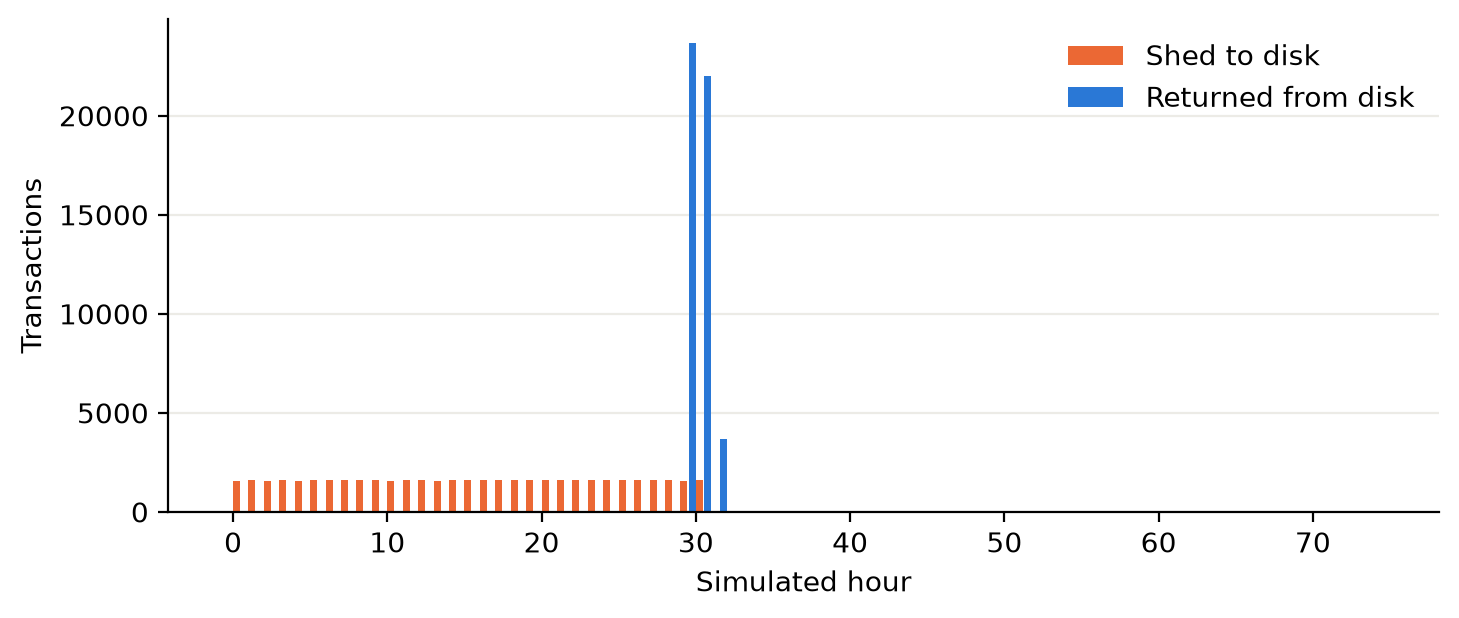
\includegraphics[width=0.85\textwidth]{figures/shed.png}
  \caption{Transactions shed and returned in each simulated hour of the official run.}
  \label{fig:shed}
\end{figure}

\subsection{Group by group}

<<T:groups>>

\subsection{Reconciliation}

By the end of the official run the warehouse held <<n:fact.rows_loaded>> transactions, with quantity <<n:fact.quantity>> and revenue <<f3:fact.revenue>>.

<<T:routes>>

<<T:left_over>>

% ------------------------------------------------------------------ 9
\section{OLAP Analysis}
\label{sec:olap}

The script \code{Queries-DW/queries_dw.sql} answers all 20 questions from the DW Analysis section, using the stored revenue. Slicing appears in Q4, Q9, Q10, Q12 and Q18, which fix time at 2011, and dicing in Q1, Q6 and Q11. Drill-down appears in Q1 and Q9 (year to month), Q13 (store to supplier to product), Q14 (product to season), Q17 (grand total to product) and Q19 (product to day). MySQL does not support materialized views, and the assignment rules out storing totals in a second fact table, so Q20 is a plain view, with the ordering applied by the \texttt{SELECT} that reads it.

Each query's output was checked row by row, with exact decimals, against answers calculated independently in pandas from the raw file.

\subsection{Reading the results}

Several features of the data affect how the results should be read. The loaded year is 2011, because 2010 has only December. December 2011 stops on the 9th, so that month and Q4 2011 are partial, and their growth figures look artificially low. The cleaned data has no Saturday transactions, so weekend means Sunday (62,773 rows).

Revenue is overstated, because cleaning removes cancellation lines but keeps the sales they cancelled. The removed lines are worth 611,342.09, or 6.86\% of cleaned revenue. The clearest case is product 23843, which ranks first overall because of a single line of 80,995 units worth 168,469.60, cancelled 12 minutes later. Six non-merchandise codes (POST, M, DOT, C2, PADS and BANK CHARGES) also remain as products, with 1,547 rows and 150,341.25 in revenue.

For Q16, the top pairs by distinct carts are (22386, 85099B) in 546 carts, (22697, 22699) in 541, (22726, 22727) in 530, (20725, 22384) in 523 and (20725, 22383) in 519. These pairs could be used for product bundles.

\subsection{Q19: comment on the revenue spikes}

Q19 finds <<n:q19.spike_days>> spike days across <<n:q19.products>> products, out of <<n:q19.product_days>> product-days with sales. Each product's average is taken over the days it actually sold. The five largest spikes, measured as a multiple of the product's own average, are listed in Table~\ref{tab:spikes}.

<<T:spikes>>

The spikes fall into three groups. Some are data errors that look like demand: product 23166 reached 77,183.60 on 18 January 2011, about 109 times its average, from a single 74,215-unit order that was cancelled 16 minutes later. Others come from single large lines: product 22502 reached about 94 times its average on 10 June 2011, mostly from one line of 60 units at 649.50, worth 38,970.00, which should be checked before it is taken at face value. The third group is seasonal. Spike days cluster between September and November 2011 (<<m:2011-09>>, <<m:2011-10>> and <<m:2011-11>>), which fits stock-buying for Christmas.

The rule also has a blind spot. Product 23843 has the largest line in the file but is never flagged, because it sold on only one day, so that day's revenue equals its own average. The test compares each product with its own history, and a product with no history cannot exceed it.

\subsection{Query run times}

<<T:timings>>

Timings were measured on database \code{<<e2:olap.database>>} with a stock MySQL 8.0 configuration and a 128~MB buffer pool. The slowest query took <<e2:olap.slowest_seconds>> seconds. Q16 needed extra work: a plain self join produced 9.8 million pair rows and ran for over two minutes on this server. Since a pair cannot appear in more carts than either of its products, the 5th best pair among the 100 most frequent products sets a floor, and only products in at least that many carts need to be paired. The answer is still exact, and it was checked against the independent calculation.

% ------------------------------------------------------------------ 10
\section{Bonus: The Live Cache}

The bonus only changes when a Live result enters the warehouse. Fully enriched Live join results are written to the \code{live_cache} table. During a slow period, which this project takes to mean non-peak speed, they are copied through the same loader as every other path, and the copied rows are deleted in the same transaction, so a row is always in exactly one place. Periodic results are never cached and still load on the hour after they are joined. The cache is also emptied when the program closes, so no row is stranded. Starting the program with \texttt{-{}-live-load direct} sends Live results straight into the fact table instead.

% ------------------------------------------------------------------ 11
\section{Testing and Verification}

<<T:tests_intro>>

<<T:tests>>

The engine is tested for every combination of the two cursors' positions, including a test that fails if a chunk leaves one iteration early. The real program also runs as a child process, with commands typed into it through standard input, in every mode. It was killed outright twice mid-run and then resumed, and a row-by-row comparison of the fact table with the source showed no row lost or doubled. All of its database connections were killed repeatedly during a run, and it recovered on its own with exact totals. Further tests check that the password never appears in output, logs or source files.


% ------------------------------------------------------------------ 12
\section{Interpretations of the Assignment}

Where the assignment leaves a point open, the program uses the readings below. These are my interpretations, not requirements of the assignment.

\begin{longtable}{@{}>{\raggedright\arraybackslash}p{5.6cm}>{\raggedright\arraybackslash}p{9.2cm}@{}}
\caption{Interpretations used where the assignment is open or ambiguous.}\\
\toprule \textbf{Point} & \textbf{Reading used} \\ \midrule \endfirsthead
\toprule \textbf{Point} & \textbf{Reading used} \\ \midrule \endhead
\bottomrule \endfoot
    \code{processing_mode}, named in section 6.2 and never defined & The route the row took: Live, Periodic or Shed. \\
    Where the store is added (sections 4.2 and 5.4.3 differ) & Outside MESHJOIN, from the in-memory \code{Store_list}. \\
    Materialized view (section 11) and view (Q20) & A plain view, for the reasons in Section~\ref{sec:olap} of this report. \\
    The loaded year & 2011. December 2010 and Q4 2010 are the base for the first growth figures. \\
    Q1 and Q11 & Q1 ranks over the whole year, then drills into months. Q11 ranks inside each month. \\
    When MESHJOIN cannot cope & At peak, periodic rows that do not fit the stream buffer when their group is released. \\
    Longest Description & Trim edge spaces, then take the longest; the first in file order wins a tie (54 products tie). \\
    Shed rows in online mode & They stay on disk, because that mode is online form only. \\
    Slow period & Non-peak speed, plus a final flush when the program closes. \\
    Q7 and Q19 averages & Q7 per transaction, with a per-cart column. Q19 over the days the product sold. \\
    Age group labels & ASCII hyphens, such as \code{0-17}, instead of en dashes. \\
\end{longtable}

% ------------------------------------------------------------------ 13
\section{Lessons Learned}

Rules that look simple depend on exact text. A single decimal point in a customer id would have quietly changed every derived attribute without raising an error, and checking the rules against known values caught this before any data was loaded. Natural keys need the same scrutiny: the obvious key for the fact table is not unique, and enforcing it would have lost rows without any warning.

Averages and quick arithmetic hid problems until they were measured. The join had plenty of capacity for the average arrival rate, yet the hourly burst still forced shedding, so the shape of the load mattered more than its rate. The store skew came from reusing one number for two remainders, and it appeared only once the carts were counted.

Checking the results needed an independent method. An early float-based profile gave 22,887 spike days for Q19, while exact arithmetic gave 22,885, because 34 product-days sit at exactly twice their average. Recomputing every answer separately found mistakes in the checks themselves as well as in the numbers. The cleaning rules also shaped the analysis: they kept sales that were cancelled minutes later, and the warehouse's top product is one of them, so totals are only as meaningful as the cleaning behind them.

% ------------------------------------------------------------------ 14
\section{Dataset Citation}

The transactional data comes from the UCI Machine Learning Repository \cite{chen}, downloaded on 3 November 2026 from \url{https://archive.ics.uci.edu/dataset/352/online+retail}.

\begin{thebibliography}{9}
  \bibitem{chen} D.~Chen, S.~L.~Sain and K.~Guo. \emph{Online Retail}. UCI Machine Learning Repository. \url{https://archive.ics.uci.edu/dataset/352/online+retail}. Downloaded 3 November 2026.
  \bibitem{polyzotis} N.~Polyzotis, S.~Skiadopoulos, P.~Vassiliadis, A.~Simitsis and N.-E.~Frantzell. Meshing Streaming Updates with Persistent Data in an Active Data Warehouse. \emph{IEEE Transactions on Knowledge and Data Engineering}, 2008.
\end{thebibliography}

\end{document}
